\section{Allgemeine Potenzreihenl"osung}

\begin{equation}
	y''+\sum_{i=0}^{n}\lambda_ix^i y=0, \quad n \ge 0
	\label{eq:wellen:allgemeinesproblem}
\end{equation}

Aufgrund der bisherigen Beobachtungen ist es nun m"oglich, eine 
allgemein geltende Potenzreihenl"osung f"ur diese Art Differentialgleichungen 
zu erstellen.

Hierzu wird die anf"angliche Parabel $ax^2 + bx + c$ mit dem allgemeinen Polynom
\begin{equation*}
	\lambda_nx^n + \lambda_{n-1}x^{n-1} + \lambda_{n-2}x^{n-2} + \dotsb + 
	\lambda_2x^2 + \lambda_1x + \lambda_0 = \sum_{i=0}^{n}\lambda_ix^i, \quad n 
	\ge 0
\end{equation*}
ersetzt.

Bei der neuen Problemstellung handelt es sich immernoch um eine 
Differentialgleichungen zweiter Ordnung. Es bleibt also eine Abh"angigkeit von 
mindestens zwei zwischen den verschiedenen $a_k$. Zus"atzlich erh"oht sich 
diese jeweils um den Polynomkoeffizientenindex. Daraus folgt nun
\begin{equation*}
	a_k = -\frac{1}{k(k-1)}\sum_{i=0}^{n}a_{k-2-i)}\lambda_i, \quad n \ge 0, 
	a_{k-2-i < 0} =  0.
\end{equation*}
f"ur ein Polynom $n$-ten Grades.

Die Potenzreihenl"osung f"ur \ref{eq:wellen:allgemeinesproblem} lautet somit:
\begin{equation}
	y(x) = a_0 + a_1x - \sum_{k=2}^{\infty}\frac{1}{k(k-1)}\sum_{i=0}^{n}
	\lambda_ia_{k-2-i}x^k, \quad n \ge 0, a_{k < 0} = 0
	\label{eq:wellen:allgemeineloesung}
\end{equation}

\subsection{Schlussfolgerungen}

Mit der Formel \ref{eq:wellen:allgemeineloesung} gibt es nun ein einfaches 
Werkzeug mit dem man allein durch Einsetzen die Potenzreihenl"osung f"ur 
diese Art von Differentialgleichungen erh"alt.

Sie erlaubt es uns aber auch noch weitere Schl"usse zu ziehen. So kann man 
nun direkt aus der Form der L"osung des gegebenen Polynoms ablesen, wie sich 
die Differentialgleichung verhalten wird. Soll heissen, positive L"osungen 
f"uhren zu einer Wellenform, die $\sin$ und $\cos$ enthalten. Negative 
L"osungen liefern hingegen eine Kombination aus $\sinh$ und $\cosh$.

\subsection{Berechnungsaufwand}
Der Pseudocodes \ref{alg:wellen:potenzreihenrechnung} kann mit kleinen 
"Anderungen an die neue L"osung angepasst werden. Es ergibt sich somit der 
Pseudocode f"ur die allgemeine Potenzreihenl"osung dieser Differentialgleichung 
\ref{alg:wellen:allgemeinepotenzreihenrechnung}.

\begin{algorithm}
	\floatname{algorithm}{Pseudocode}
	\begin{algorithmic}[1]
		\State $i \gets 1$
		\State $a_{k<0} \gets 0$
		\State $a_0 \gets y(0)$
		\State $a_1 \gets y'(0)$
		\State $x \gets x_{\text{min}}$
		\For{$x \le x_{\text{max}}$}
			\State $k \gets 2$
			\State $\text{sum} \gets a_0 + a_1x$
			\For{$k \le k_{\text{max}}$}
				\State $i \gets 0$
				\State $\text{aksum} \gets 0$
				\For{$i \le n$}
					\State $\text{aksum} \gets \text{aksum}+\lambda_i a_{k-2-i}$
					\State $i \gets i + 1$
				\EndFor
				\State $a_k \gets -\frac{1}{k(k-1)} \cdot \text{aksum}$
				\State $\text{sum} \gets \text{sum} + a_k x^k$
				\State $k \gets k + 1$
			\EndFor
			\State $x \gets x + x_{\text{step}}$
		\EndFor
	\end{algorithmic}
	\caption{Allgemeine Potenzreihenberechnung} 
	\label{alg:wellen:allgemeinepotenzreihenrechnung}
\end{algorithm}

Der allgemeine Algorithmus hat also eine Laufzeit von
\begin{equation*}
\mathcal{O}\left(nk_{\text{max}}\frac{x_{\text{max}}-x_{\text{min}}} 
{x_{\text{step}}}\right),
\end{equation*}
wobei $n$ dem Grad des gegebenen Polynoms entspricht.

\subsection{Beispiel: \texorpdfstring{$n = 1$}{n = 1}, 
Airy-Differentialgleichung}
Die bereits bekannte Airy-Differentialgleichung
\begin{align*}
	y''-xy = 0
\end{align*}
ergibt nun in die allgemeine L"osungsformel \ref{eq:wellen:allgemeineloesung} 
eingesetzt

\begin{equation*}
\begin{split}
	y(x) &= a_0+a_1x-\sum_{k=2}^{\infty} \frac{1}{k(k-1)} ((-1) a_{k-2-1} + 0 
	a_{k-2-0}) x^k
	\\
	&= a_0+a_1x+\sum_{k=2}^{\infty} \frac{1}{k(k-1)} a_{k-3} x^k,
	\qquad a_{k < 0} = 0,
\end{split}
\end{equation*}
was sich mit den bereits bekannten L"osung deckt.

Graphisch betrachtet werden die genannten Konsequenzen deutlich erkennbar:

\begin{center}
	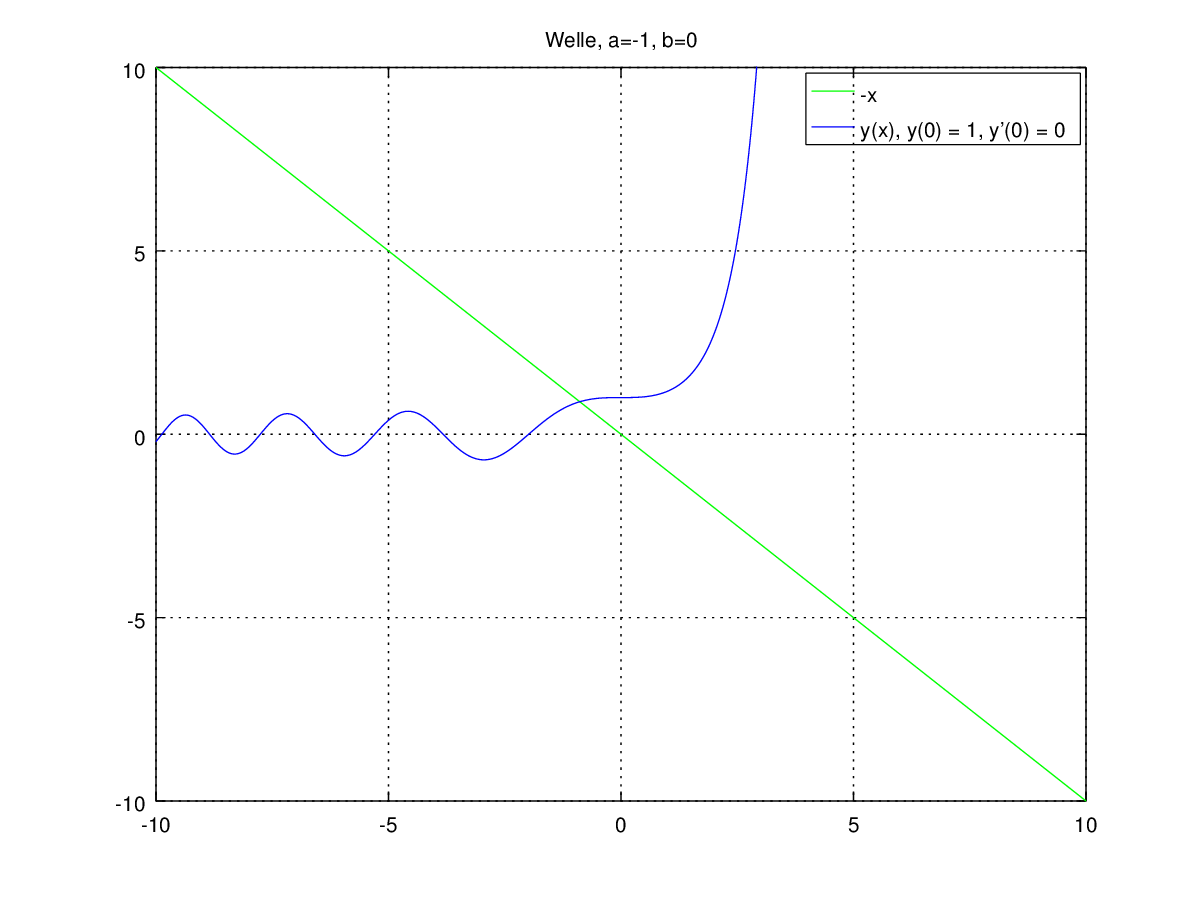
\includegraphics[scale=0.65]{./wellen/images/allgemein/n1.png}
\end{center}

\subsection{Beispiel: \texorpdfstring{$n = 4$}{n = 4}}

Auch ein Polynom 4-ten Grades stellt kein Problem dar. Die 
Differentialgleichung:

\begin{equation*}
	y''+(ax^4+bx^3+cx^2+dx+e)y = 0
\end{equation*}
ergibt nach dem Einsetzen:

\begin{align*}
	y(x) &= a_0+a_1x-\sum_{k=2}^{\infty} \frac{1}{k(k-1)} (aa_{k-2-4} + 
	ba_{k-2-3} + ca_{k-2-2} + da_{k-2-1} +ea_{k-2-0})x^k
	\\
	&= a_0+a_1x-\sum_{k=2}^{\infty} \frac{1}{k(k-1)} (aa_{k-6} + ba_{k-5} + 
	ca_{k-4} + da_{k-3} +ea_{k-2})x^k, \qquad a_{k<0} = 0
\end{align*}

Auch hier kann man graphisch die "Uberg"ange zwischen $\sin$ und $\cos$ bei 
positiven und $\sinh$ und $\cosh$ bei negativen Polynoml"osungen klar erkennen.

\begin{center}
	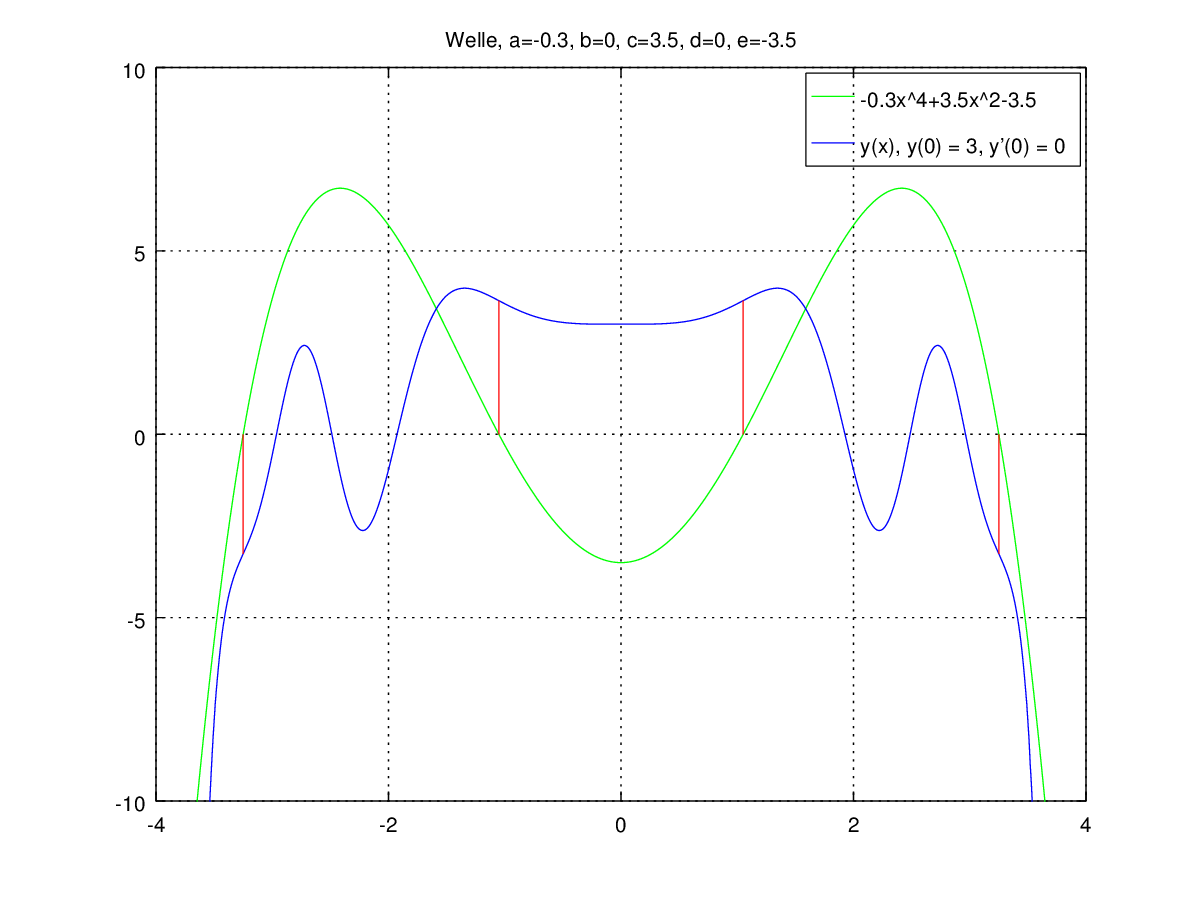
\includegraphics[scale=0.65]{./wellen/images/allgemein/n4.png}
\end{center}